\chapter{Literature Review}
\label{chap:literature_review}

\section{Overview}
The design of an Agentic AI Tutor builds on several modern AI concepts: Small Language Models (SLMs), Retrieval-Augmented Generation (RAG), and MLOps practices for deployment.

This chapter reviews academic and technical literature that informs the design of the Agentic AI Tutor. It focuses on Large and Small Language Models (LLMs and SLMs) in educational contexts, summarises benefits and challenges, and motivates the use of smaller, modular, and explainable systems.

\section{Premiere in LLM for Education}

\subsection{What are the models}
Language models are neural networks that learn to predict the next word (token) in a text. They work on sequences of tokens and update millions of internal parameters (weights) during training. The number of parameters is a simple way to describe model size and capacity: more parameters allow the model to store and combine more patterns, but also make training and serving much more expensive.

Language models use the transformer architecture. During training, text is split into tokens; the model predicts the next token and adjusts its parameters to reduce error.

\subsection{Fundamentals of Transformer Models}
Modern Large and Small Language Models are based on the Transformer architecture introduced by Vaswani et al. \parencite{Untitled54:online}. Instead of recurrent or convolutional layers, the Transformer uses multi-head self-attention, where each token can attend to all other tokens in the sequence. This design makes long-range dependencies easier to learn and allows full parallelisation during training. Positional encodings are added to token embeddings so that the model can still represent word order without recurrence.

\subsection{Types of language models}

\textbf{Large Language Models (LLMs)} (e.g., GPT or Claude) have billions to trillions of parameters and are trained on web-scale data. They offer broad knowledge and strong general reasoning, but they usually need datacenter GPUs and cloud APIs to run \parencite{LLMVsSLM66:online}.

\textbf{Small Language Models (SLMs)} are compact transformer models with up to \(\approx 10\)B. They focus on narrower tasks or domains. SLMs can run on a single consumer GPU or even on edge devices with low latency and lower energy use \parencite{SmallLan73:online,LLMVsSLM66:online}.

The main practical difference is that LLMs have more parameters, which increases memory, compute, and cost.

\subsection{Operational differences that matter}

In practice, developers choose between LLMs and SLMs by looking at three things: compute, deployment, and training data.

\paragraph{Compute and cost}
Serving a 7B SLM can be about 10-30 times cheaper (in latency, energy consumption, and FLOPs) than serving a 70-175B LLM, while keeping similar accuracy on focused tasks. SLMs usually run on one GPU without parallelism; LLMs often need multi-GPU setups \parencite{SmallLan73:online}.

\paragraph{Deployment}
LLMs are commonly offered as centralised cloud APIs with heavy backends. SLMs fit well into local or edge microservices and can be embedded inside products or agents with tight latency budgets \parencite{LLMVsSLM66:online,SmallLan73:online}.

\paragraph{Training data and adaptation}
LLMs are trained on massive, diverse datasets and are strong at open-domain tasks.
SLMs can be fine-tuned faster and cheaper on smaller, domain-specific datasets (for example, one subject or one product line), which is useful for modular agent systems and on-device scenarios \parencite{LLMVsSLM66:online,SmallLan73:online}.

\begin{table}[h]
\centering
\caption{LLMs vs.\ SLMs: practical differences for this project (adapted from \cite{LLMVsSLM66:online,SmallLan73:online}).}
\label{tab:llm-slm}
\begin{tabular}{p{0.32\linewidth} p{0.28\linewidth} p{0.28\linewidth}}
\toprule
\textbf{Dimension} & \textbf{LLMs} & \textbf{SLMs} \\ \midrule
Typical size & Billions-trillions of params & Millions-10B params \\
Compute cost & Very high; often multi-GPU & Low; single GPU \\
Latency & Higher (network + compute) & Low; real-time friendly \\
Deployment & Cloud APIs, heavy backends & Local/edge microservices \\
Training data & Web-scale, very diverse & Smaller, domain-specific \\
Adaptation speed & Slower, costly & Faster; PEFT/LoRA friendly \\
Energy/CO\textsubscript{2} & High footprint & Up to 10-30 times lower \\
Best for & Broad knowledge, open tasks & Focused tasks, modular agents \\
\bottomrule
\end{tabular}
\end{table}
\FloatBarrier

\subsection{Premiere Applications of LLMs in education}
The integration of Large Language Models (LLMs) into education began shortly after the public release of ChatGPT in late 2022. As reported by Guizani et al. (2025), the adoption of LLMs such as GPT-3 and GPT-4 has transformed educational practices by enabling automated grading, interactive tutoring, and personalized learning experiences \parencite{Asystema7:online}. Early case studies in universities and online platforms demonstrated that LLMs could improve engagement and accessibility, supporting language learning, summarisation, and formative feedback \parencite{ChatGPTf63:online}. However, this first wave of integration also raised concerns about reliability, bias, and academic integrity, prompting educators and policymakers to establish initial guidelines for ethical use \parencite{Untitled13:online, Practica79:online}. The concept of an educational overview for non-experts for LLMs has been explored by Idan and Einav (2025), who presented an accessible framework for understanding LLM architecture, including embeddings, tokens, and transformer layers \parencite{Primeron58:online}. Although written for clinical practitioners, their approach illustrates how LLMs can serve as educational tools themselves by providing clear explanations and acting as teaching partners. This reflects a broader movement towards AI literacy and the responsible introduction of LLMs into professional learning contexts.

\subsection{Real-world Applications of LLMs in Education}

\paragraph{Khanmigo (Khan Academy)}
Khanmigo is an AI-powered tutor described as "a tutor for learners and an assistant for teachers." It provides personalised guidance in mathematics, science, and humanities, acts as a debate or writing coach, and can simulate historical figures for contextual learning. For teachers, it helps design rubrics, plan lessons, and generate feedback. Khanmigo’s pedagogical design focuses on guided questioning rather than giving direct answers, encouraging critical thinking and problem solving \parencite{Khanmigo61:online}. However, human oversight remains essential to verify factual accuracy and moderate potential bias.

\paragraph{Duolingo Max}
Launched in 2023, Duolingo Max integrates OpenAI’s GPT-4 into its premium subscription tier, adding two key features: Explain My Answer and Roleplay. The first explains grammatical or conceptual errors immediately after exercises, while the second lets learners practise real-world dialogues (e.g., ordering coffee, planning trips) with AI characters that give instant feedback on accuracy and complexity. Both modes were refined through close collaboration with OpenAI and reviewed by human curriculum experts to ensure correctness and tone \parencite{Duolingo46:online}. This model demonstrates how LLMs can enhance adaptive, feedback-driven, and motivational language learning at scale.

\paragraph{Quizlet Q-Chat}
Quizlet’s Q-Chat, introduced in 2023, was the first fully adaptive conversational tutor built on the ChatGPT API and integrated with Quizlet’s extensive study library. It follows the Socratic method (ask progressively deeper questions rather than providing direct answers) to promote active recall and conceptual understanding. Q-Chat personalises interactions according to the learner’s subject, level, and progress, enabling dynamic question generation from structured study sets. Q-Chat exemplified how LLMs could provide affordable, scalable tutoring aligned with sound pedagogical principles \parencite{Introduc91:online}.


\paragraph{From promise to practicality}
While these examples demonstrate the transformative potential of LLMs in education, they also expose important limitations for sustainable adoption.  
All three systems: Khanmigo, Duolingo Max, and Q-Chat, rely on cloud-hosted proprietary models such as GPT-4, which require constant internet access, high subscription costs, and centralised data handling \parencite{Khanmigo61:online, Duolingo46:online, Introduc91:online}. This dependency raises issues of privacy, transparency, and accessibility, particularly for institutions with limited computational or financial resources \parencite{Untitled13:online, ChatGPTf63:online, Practica79:online}. Moreover, the pedagogical success of these systems depends heavily on human curation and oversight, which reduces scalability \parencite{Duolingo46:online, Khanmigo61:online, ChatGPTf63:online}. Therefore, despite their achievements, LLM-based platforms highlight the need for more lightweight, explainable, and modular solutions requirements that motivate the use of Small Language Models (SLMs) and agentic architectures in this project \parencite{SmallLan73:online, LLMVsSLM66:online}.


\section{Challenges of LLMs in Education}
Despite their strong reasoning abilities, LLMs face several pedagogical, ethical, and technical limitations that restrict their use in education. A systematic review by Guizani et al. (2025) and Yan et al. (2024) identifies recurring concerns such as bias, misinformation, and the risk of over-reliance on automated feedback \parencite{Asystema7:online, Practica79:online}. Educators also report difficulties verifying AI-generated content and maintaining transparency in assessment \parencite{ChatGPTf63:online}. From a policy perspective, the UK Department for Education (2024) calls for stronger ethical guidance, data governance, and teacher training before large-scale adoption \parencite{Untitled13:online}.

Beyond ethical and pedagogical issues, LLMs also pose serious resource challenges.  
They require high-end GPUs, large-scale cloud infrastructure, and significant financial and energy costs to operate. Training and deploying models exceeding 70B parameters may generate substantial carbon emissions and limit access for institutions with modest resources \parencite{SmallLan73:online, LLMVsSLM66:online}. Latency, dependency on external APIs, and privacy risks associated with cloud-based inference further constrain their usability in schools and universities. These limitations make LLMs powerful but impractical for real-world, low-resource educational settings.

\subsection{Hallucinations in Large Language Models}
Another major technical and pedagogical limitation of large models is their tendency to produce hallucinations. According to Huang et al. (2024), hallucinations in LLMs can be grouped into two main categories:factuality, when the model outputs text that conflicts with verifiable real-world facts, and faithfulness, when the output deviates from the user’s instruction, provided context, or the model’s own reasoning chain \parencite{Huang2024HallucinationSurvey}.  

The survey identifies three main sources of hallucination: (1) noisy or biased training data,  
(2) imperfect alignment during fine-tuning, and (3) exposure bias and sampling errors at inference time.  
In educational contexts, these errors can mislead learners by generating plausible but incorrect explanations or references. As a mitigation strategy, researchers increasingly combine generation with external knowledge retrieval, known as Retrieval-Augmented Generation (RAG), to verify or ground the model’s outputs. However, as noted by Huang et al. (2024), RAG itself is not a complete solution:  
it reduces factuality errors but may still suffer from faithfulness violations if the retrieved evidence is ignored or misinterpreted.

In summary, the challenges of LLMs can be grouped into four categories:
\begin{itemize}
    \item \textbf{Ethical and legal:} bias, privacy, transparency, and academic integrity \parencite{Practica79:online, Dataprot22:online, CodeofEt55:online};
    \item \textbf{Pedagogical:} reduced critical thinking and over-reliance on automated support \parencite{ChatGPTf63:online, Primeron58:online};
    \item \textbf{Technical and resource-related:} cost, energy, latency, and accessibility barriers \parencite{SmallLan73:online, LLMVsSLM66:online};
    \item \textbf{Epistemic:} hallucinations and unreliability of generated information, where outputs appear fluent but lack factual accuracy or deviate from instructions and context  
    \parencite{Huang2024HallucinationSurvey}.
\end{itemize}

Together, four factors highlight why monolithic LLM architectures are often unsuitable for sustainable educational deployment.

\subsection{Small Language Models (SLMs)}

Recent studies show that Small Language Models (SLMs) can now achieve accuracy close to Large Language Models (LLMs) while using much less computing power.
According to \parencite{240915795:online}, SLMs are designed for efficient use on personal devices such as laptops, smartphones, and IoT systems.
They can perform reasoning and problem-solving tasks with good accuracy while keeping memory and latency low.

The 2024 survey by Lu et al. compared 70 open-source SLMs from 100 million to 5 billion parameters and found that small models such as Phi, Gemma, and Qwen perform almost as well as larger LLaMA models. The paper highlights three main reasons for this progress: (1) improved architectures like grouped-query attention and gated feed-forward networks, (2) higher-quality filtered datasets such as FineWeb-Edu and DCLM, and (3) hardware-aware quantisation that enables on-device inference.

A new January 2025 survey confirms this trend \parencite{2501054671:online}.
It reviews 160 papers and shows that SLMs with 1-8 billion parameters can now rival or even surpass much larger LLMs on many benchmarks.
The authors note that 7B-parameter models can train or run on a single consumer GPU (for example, RTX 4090), which fits student-level resources such as Google Colab. This supports the decision to select a compact open-source model with up to 7B-parameter instead of running costly distillation.

Figure \ref{fig:slm_timeline} illustrates the key milestones in the evolution of open-source Small Language Models (SLMs), showing how efficiency-oriented architectures emerged between 2022 and 2025.

\begin{figure}[h]
  \centering
  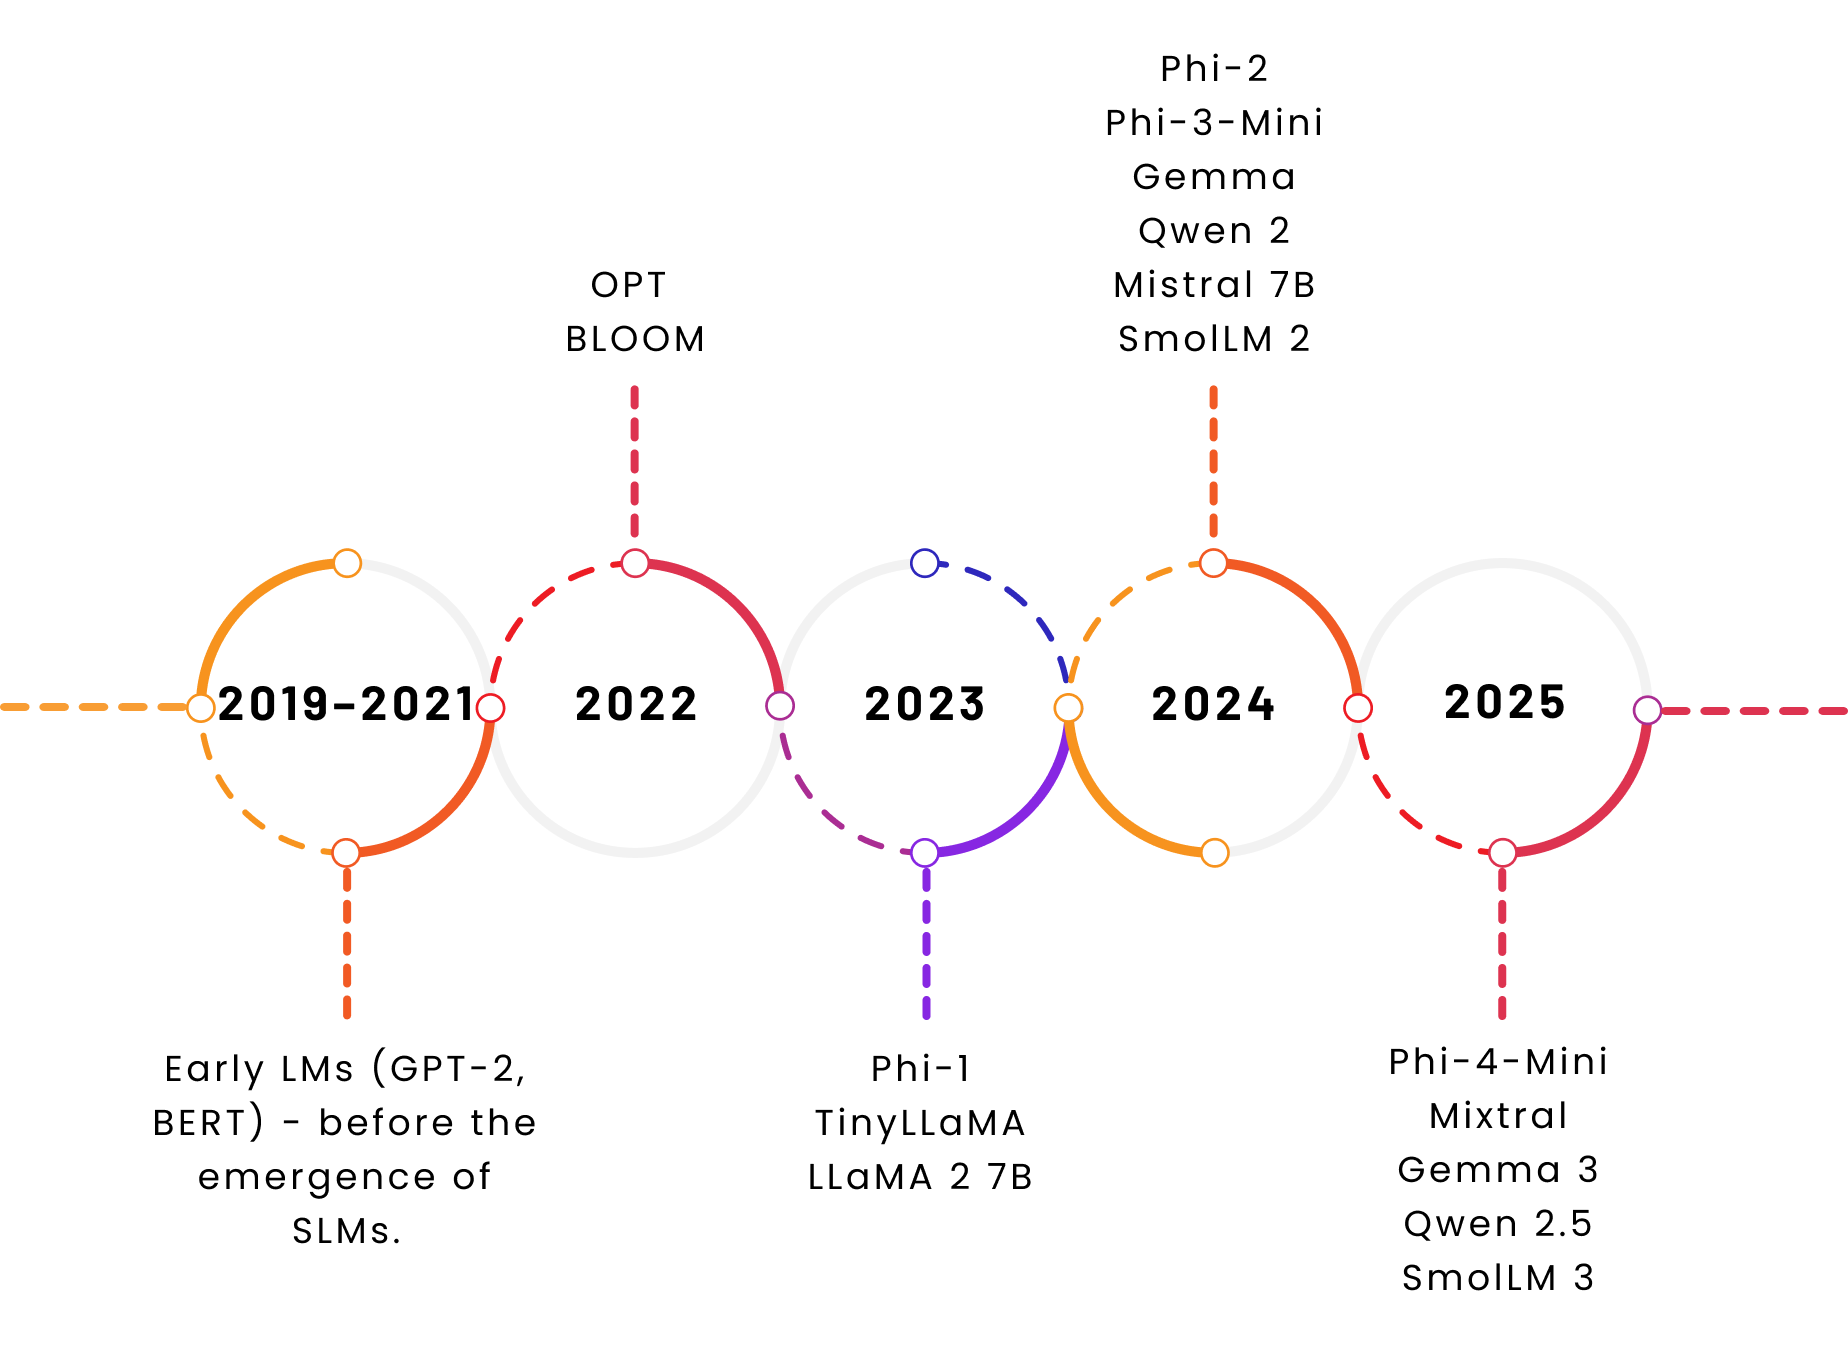
\includegraphics[width=\linewidth]{figs/slm_timeline_combined.png}
  \caption{Evolution of Small Language Models (SLMs) from 2019 to 2025. 
  The timeline highlights key open-source models that shaped the development of efficient AI systems.}
  \label{fig:slm_timeline}
\end{figure}

\section{How SLMs and Agentic AI Address These Challenges}
Small Language Models (SLMs) and modular agentic architectures offer a practical and sustainable response to these limitations. SLMs maintain the same transformer-based reasoning mechanism as LLMs but are trained on smaller, curated datasets. This makes them faster to adapt, cheaper to deploy, and easier to control \parencite{SmallLan73:online, 240915795:online}. Because SLMs can run locally or on low-power GPUs, they support educational institutions with limited budgets or infrastructure while complying with data protection standards \parencite{Dataprot22:online}.

In contrast to single, opaque LLMs, \textit{Agentic AI} distributes intelligence across multiple smaller agents. Each agent performs a focused role such as retrieval, reasoning, feedback generation, or assessment, and communicates with others through defined APIs. This modular approach improves transparency and allows fine-grained supervision: teachers or administrators can monitor each component’s outputs independently. According to NVIDIA Research, SLM-based agentic systems are more efficient and scalable for repetitive or structured subtasks \parencite{SmallLan73:online}. In education, this translates into specialised subject agents, explainable reasoning paths, and real-time collaboration between human and AI components.

By combining SLM efficiency with agentic modularity, educational AI can evolve from large, opaque systems toward distributed, explainable, and sustainable architectures. This approach directly addresses the cost, energy, and trust challenges of LLMs while maintaining pedagogical flexibility and human oversight.

In our design, subject-specific SLM agents (fine-tuned or adapted via PEFT/LoRA) are orchestrated with retrieval and evaluation agents, yielding lower latency and cost while enabling auditable, teacher-in-the-loop workflows \parencite{SmallLan73:online,2106096835:online}.

To address these challenges in practice, a set of dedicated development and orchestration tools will be introduced and examined in the following chapter.